\documentclass[tikz,border=2mm]{standalone}

\begin{document}
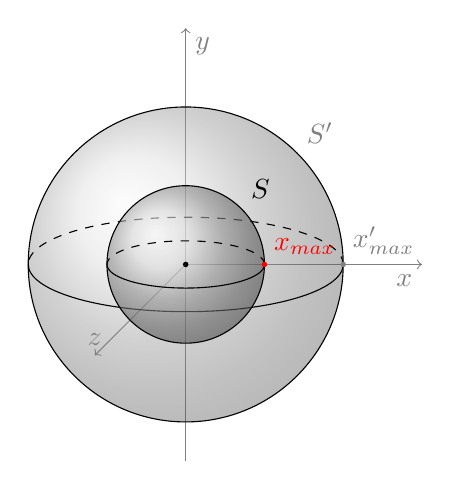
\begin{tikzpicture}

\draw[->, color=gray] (0,0,0) -- (3,0,0) node[anchor=north east]{$x$};
\draw[->, color=gray] (0,-2.5,0) -- (0,3,0) node[anchor=north west]{$y$};
\draw[->, color=gray] (0,0,0) -- (0,0,3) node[anchor=south]{$z$};

\shade[ball color = gray!40, opacity = 0.4] (0,0) circle (2);
\draw (0,0) circle (2);
\draw (-2,0) arc (180:360:2 and 0.6);
\draw[dashed] (2,0) arc (0:180:2 and 0.6);

\shade[ball color = gray!40, opacity = 0.6] (0,0) circle (1);
\draw (0,0) circle (1);
\draw (-1,0) arc (180:360:1 and 0.3);
\draw[dashed] (1,0) arc (0:180:1 and 0.3);

\fill ({cos(45)},{sin(45)},0) circle (0pt) node[anchor=south west]{$S$};
\fill ({2*cos(45)},{2*sin(45)},0) circle (0pt) node[anchor=south west, gray]{$S'$};

\fill[fill=black] (0,0,0) circle (1pt);
\fill[fill=red] (1,0,0) circle (1pt) node[anchor=south west, red]{$x_{max}$};
\fill[fill=gray] (2,0,0) circle (1pt) node[anchor=south west, gray]{$x'_{max}$};

\end{tikzpicture}
\end{document}